\documentclass{zkdl-presentation-template}

\usepackage[dvipsnames]{xcolor}

\title[zk-SNARK I]{\textbf{QAP, PCP, POE}}
\author{Distributed Lab}
\date{Oct 1, 2024}
\titlegraphic{
    
\includegraphics[width=\textwidth]{images/banner_wide.png}
}

\begin{document}
    \frame {
        \titlepage
    }

    \begin{frame}{Plan}
        \tableofcontents
    \end{frame}

    \section{Recap}

    \begin{frame}{Recap. ZK-SNARK}
        \begin{definition}
            \textbf{zk-SNARK} – Zero-Knowledge Succinct Non-interactive ARgument of 
            Knowledge.
        \end{definition}
        \pause
        \begin{itemize}[itemsep=1pt]
            \item \textbf{Argument of Knowledge} --- a proof that the prover knows the data (witness) that resolves a certain
            problem, and this knowledge can be ``extracted''. \pause
            \item \textbf{Succinctness} --- the proof size and verification time is relatively small to the computation size and typically does not depend on the size of 
            the data or statement. \pause
            \item \textbf{Non-interactiveness} --- to produce the proof, the prover does not need any interaction
            with the verifier. \pause
            \item \textbf{Zero-Knowledge} --- the verifier learns nothing about the data used to produce the
            proof, despite knowing that this data resolves the given problem and that the prover possesses it.
        \end{itemize}
    \end{frame}

    \begin{frame}{Recap. Arbitrary Program To Circuits}
        We can do that in a way like the computer does it - boolean circuits.

        % --- Writing diagrams ---
        % Define circle styles and colors
        \colorlet{circle edge}{gray!50!black}
        \colorlet{circle area}{gray!20}
        \colorlet{gate1 edge}{green!50!black}
        \colorlet{gate1 area}{green!20}
        \colorlet{gate2 edge}{orange!50!black}
        \colorlet{gate2 area}{orange!20}
        \colorlet{gate3 edge}{blue!50!black}
        \colorlet{gate3 area}{blue!20}

        \tikzset{
            var/.style={circle, draw=circle edge, fill=circle area, very thick, minimum size=0.7cm, text centered},
            gate1/.style={circle, draw=gate1 edge, fill=gate1 area, ultra thick, minimum size=1cm, text centered},
            gate2/.style={circle, draw=gate2 edge, fill=gate2 area, ultra thick, minimum size=1cm, text centered},
            gate3/.style={circle, draw=gate3 edge, fill=gate3 area, ultra thick, minimum size=1cm, text centered},
            arrow/.style={-latex, ultra thick}
        }

        \begin{figure}[h!]
            \centering
            
            \begin{minipage}{0.54\textwidth}
                \centering
                % Boolean AND and OR gates
                \begin{tabular}{cc}
                    \begin{tikzpicture}
                        % Nodes
                        \node[var] (a) at (0, -1.5) {$a$};
                        \node[var] (b) at (2, -1.5) {$b$};
                        \node[gate1] (and) at (1, 0) {\texttt{AND}};
                        \node[var] (c) at (1, 1.75) {$c$};
        
                        % Arrows
                        \draw[arrow,gray] (a) -- (and);
                        \draw[arrow,gray] (b) -- (and);
                        \draw[arrow,gray!50!black] (and) -- (c);
                    \end{tikzpicture}
                    &
                    \begin{tikzpicture}
                        % Nodes
                        \node[var] (a) at (0, -1.5) {$a$};
                        \node[var] (b) at (2, -1.5) {$b$};
                        \node[gate2] (or) at (1, 0) {\texttt{OR}};
                        \node[var] (c) at (1, 1.75) {$c$};
        
                        % Arrows
                        \draw[arrow,gray] (a) -- (or);
                        \draw[arrow,gray] (b) -- (or);
                        \draw[arrow,gray!50!black] (or) -- (c);
                    \end{tikzpicture}
                \end{tabular}
                \centering
                \caption{Boolean \texttt{AND} and \texttt{OR} Gates}
            \end{minipage}
            \hspace{0.05\textwidth} % Space between figures
        \end{figure}

        But nothing stops us from using something more powerful instead of boolean values...
    \end{frame}

    \begin{frame}{Recap. Arbitrary Program To Circuits}
        We can do that in a way like the computer does it - boolean circuits.

        % --- Writing diagrams ---
        % Define circle styles and colors
        \colorlet{circle edge}{gray!50!black}
        \colorlet{circle area}{gray!20}
        \colorlet{gate1 edge}{green!50!black}
        \colorlet{gate1 area}{green!20}
        \colorlet{gate2 edge}{orange!50!black}
        \colorlet{gate2 area}{orange!20}
        \colorlet{gate3 edge}{blue!50!black}
        \colorlet{gate3 area}{blue!20}

        \tikzset{
            var/.style={circle, draw=circle edge, fill=circle area, very thick, minimum size=0.7cm, text centered},
            gate1/.style={circle, draw=gate1 edge, fill=gate1 area, ultra thick, minimum size=1cm, text centered},
            gate2/.style={circle, draw=gate2 edge, fill=gate2 area, ultra thick, minimum size=1cm, text centered},
            gate3/.style={circle, draw=gate3 edge, fill=gate3 area, ultra thick, minimum size=1cm, text centered},
            arrow/.style={-latex, ultra thick}
        }

        \begin{figure}[h!]
            \centering
            
            \begin{minipage}{0.54\textwidth}
                \centering
                % Boolean AND and OR gates
                \begin{tabular}{cc}
                    \begin{tikzpicture}
                        % Nodes
                        \node[var] (a) at (0, -1.5) {$a$};
                        \node[var] (b) at (2, -1.5) {$b$};
                        \node[gate1] (and) at (1, 0) {\texttt{AND}};
                        \node[var] (c) at (1, 1.75) {$c$};
        
                        % Arrows
                        \draw[arrow,gray] (a) -- (and);
                        \draw[arrow,gray] (b) -- (and);
                        \draw[arrow,gray!50!black] (and) -- (c);
                    \end{tikzpicture}
                    &
                    \begin{tikzpicture}
                        % Nodes
                        \node[var] (a) at (0, -1.5) {$a$};
                        \node[var] (b) at (2, -1.5) {$b$};
                        \node[gate2] (or) at (1, 0) {\texttt{OR}};
                        \node[var] (c) at (1, 1.75) {$c$};
        
                        % Arrows
                        \draw[arrow,gray] (a) -- (or);
                        \draw[arrow,gray] (b) -- (or);
                        \draw[arrow,gray!50!black] (or) -- (c);
                    \end{tikzpicture}
                \end{tabular}
                \centering
                \caption{Boolean \texttt{AND} and \texttt{OR} Gates}
            \end{minipage}
            \hspace{0.05\textwidth} % Space between figures
        \end{figure}
        > 100000 gates just for SHA256...
        \pause
        But nothing stops us from using something more powerful instead of boolean values, gates.
    \end{frame}

    \begin{frame}{Recap. Arbitrary Program To Circuits}
        Similar to Boolean Circuits, the \textbf{Arithmetic circuits} consist of gates and
        wires. 
        \begin{itemize}
            \item Wires: elements of some finite field $\mathbb{F}_p$.
            \item Gates: addition ($\oplus$) and multiplication ($\odot$) corresponding to the field.
        \end{itemize} 

        % --- Writing diagrams ---
        % Define circle styles and colors
        \colorlet{circle edge}{gray!50!black}
        \colorlet{circle area}{gray!20}
        \colorlet{gate1 edge}{green!50!black}
        \colorlet{gate1 area}{green!20}
        \colorlet{gate2 edge}{orange!50!black}
        \colorlet{gate2 area}{orange!20}
        \colorlet{gate3 edge}{blue!50!black}
        \colorlet{gate3 area}{blue!20}

        \tikzset{
            var/.style={circle, draw=circle edge, fill=circle area, very thick, minimum size=0.7cm, text centered},
            gate1/.style={circle, draw=gate1 edge, fill=gate1 area, ultra thick, minimum size=1cm, text centered},
            gate2/.style={circle, draw=gate2 edge, fill=gate2 area, ultra thick, minimum size=1cm, text centered},
            gate3/.style={circle, draw=gate3 edge, fill=gate3 area, ultra thick, minimum size=1cm, text centered},
            arrow/.style={-latex, ultra thick}
        }

        \begin{figure}[h!]
            \centering
            % Addition and Multiplication gates
            \begin{tabular}{cc}
                \begin{tikzpicture}
                    % Nodes
                    \node[var] (a) at (0, -1.5) {$a$};
                    \node[var] (b) at (2, -1.5) {$b$};
                    \node[gate1] (add) at (1, 0) {$+$};
                    \node[var] (c) at (1, 1.75) {$c$};

                    % Arrows
                    \draw[arrow,gray] (a) -- (add);
                    \draw[arrow,gray] (b) -- (add);
                    \draw[arrow,gray!50!black] (add) -- (c);
                \end{tikzpicture}
                &
                \begin{tikzpicture}
                    % Nodes
                    \node[var] (a) at (0, -1.5) {$a$};
                    \node[var] (b) at (2, -1.5) {$b$};
                    \node[gate2] (mul) at (1, 0) {$\times$};
                    \node[var] (c) at (1, 1.75) {$c$};

                    % Arrows
                    \draw[arrow,gray] (a) -- (mul);
                    \draw[arrow,gray] (b) -- (mul);
                    \draw[arrow,gray!50!black] (mul) -- (c);
                \end{tikzpicture}
            \end{tabular}
            \caption{Addition and Multiplication Gates}
        \end{figure}
    \end{frame}

    \begin{frame}[fragile]{Recap. Arbitrary Program To Circuits}
        \begin{example}
            How can we translate \texttt{if} statements?
            \begin{lstlisting}[language=Python, numbers=none, autogobble=true, xleftmargin=8pt]
                def example(a: bool, b: F, c: F) -> F:
                    if a:
                        return b * c 
                    else:
                        return b + c
            \end{lstlisting}
            \pause
            We can transform such a function into the next expression:
            \vspace{-8pt}
            \begin{equation*}
                r = a \times (b \times c) + (1 - a) \times (b + c)    
                \vspace{-8pt}
            \end{equation*}
            \pause
            Corresponding equations for the circuit are:
            \vspace{-8pt}
            \begin{equation*}
                \begin{aligned}
                    r_1 &= b \times c, \quad &r_3 &= 1 - a, \quad &r_5 &= r_3 \times r_2 \\
                    r_2 &= b + c, \quad &r_4 &= a \times r_1, \quad &r &= r_4 + r_5
                \end{aligned}
            \end{equation*}
        \end{example}
    \end{frame}

    \begin{frame}{Recap. Arbitrary Program To Circuits}
         % Define circle styles and colors
         \colorlet{circle edge}{gray!50!black}
         \colorlet{circle area}{gray!20}
         \colorlet{gate1 edge}{green!50!black}
         \colorlet{gate1 area}{green!20}
         \colorlet{gate2 edge}{orange!50!black}
         \colorlet{gate2 area}{orange!20}
         \colorlet{gate3 edge}{blue!50!black}
         \colorlet{gate3 area}{blue!20}
 
         \tikzset{
             var/.style={circle, draw=circle edge, fill=circle area, very thick, minimum size=0.7cm, text centered},
             gate1/.style={circle, draw=gate1 edge, fill=gate1 area, ultra thick, minimum size=1cm, text centered},
             gate2/.style={circle, draw=gate2 edge, fill=gate2 area, ultra thick, minimum size=1cm, text centered},
             gate3/.style={circle, draw=gate3 edge, fill=gate3 area, ultra thick, minimum size=1cm, text centered},
             arrow/.style={-latex, ultra thick}
         }
 
         \begin{figure}[h!]
             \centering
             \begin{tikzpicture}
                 % Nodes
                 \node[var] (c) at (0.5, -3) {$c$};
                 \node[var] (b) at (0.5, -1.5) {$b$};
                 \node[var] (a) at (0.5, 0) {$a$};
                 \node[var] (one) at (0.5, 1.5) {$1$};
         
                 % b+c and b*c gates
                 \node[gate1] (b_plus_c) at (2.5, -1.5) {$+$};
                 \node[gate2] (b_times_c) at (2.5, -3.0) {$\times$};
         
                 \node[gate3] (one_minus_a) at (2.5, 0.75) {$-$};
         
                 % a*b*c and (1-a)(b+c) gates
                 \node[gate2] (a_times_b_times_c) at (5, -2.0) {$\times$};
                 \node[gate2] (one_minus_a_times_b_plus_c) at (5, -0.5) {$\times$};
         
                 % a*b*c + (1-a)(b+c) gate
                 \node[gate1] (r) at (7.5, -1.25) {$+$};
         
                 % Result node
                 \node[var] (result) at (10, -1.25) {$r$};
         
                 % b+c and b*c arrows
                 \draw[arrow,gray] (b) to (b_plus_c);
                 \draw[arrow,gray] (b) to (b_times_c);
                 \draw[arrow,gray] (c) to (b_plus_c);
                 \draw[arrow,gray] (c) to (b_times_c);
         
                 % 1 - c arrow
                 \draw[arrow,gray] (one) to (one_minus_a);
                 \draw[arrow,gray] (a) to (one_minus_a);
         
                 % a*b*c and (1-a)(b+c) arrows
                 \draw[arrow,gray] (a) to [bend left=20] (a_times_b_times_c);
                 \draw[arrow,gray] (b_times_c) to node[midway, above] {$r_1$} (a_times_b_times_c);
                 \draw[arrow,gray] (one_minus_a) to node[midway, above] {$r_3$} (one_minus_a_times_b_plus_c);
                 \draw[arrow,gray] (b_plus_c) to node[midway, above] {$r_2$} (one_minus_a_times_b_plus_c);
         
                 % a*b*c + (1-a)(b+c) arrows
                 \draw[arrow,gray] (a_times_b_times_c) to [bend right=20] node[midway, above] {$r_4$} (r);
                 \draw[arrow,gray] (one_minus_a_times_b_plus_c) to [bend left=20] node[midway, above] {$r_5$} (r);
         
                 % Result arrow
                 \draw[arrow,gray!50!black] (r) to (result);
         
             \end{tikzpicture}
             \caption{Example of a circuit evaluating the \texttt{if} statement logic.}
             \label{fig:multivariate-polynomial-circuit}
         \end{figure}
    \end{frame}

    \begin{frame}[fragile]{Recap. Arbitrary Program To Circuits}
        \begin{example}
            How can we translate \texttt{if} statements?
            \begin{lstlisting}[language=Python, numbers=none, autogobble=true, xleftmargin=8pt]
                def example(a: bool, b: F, c: F) -> F:
                    if a:
                        return b * c 
                    else:
                        return b + c
            \end{lstlisting}
            \pause
            We can transform such a function into the next expression:
            \vspace{-8pt}
            \begin{equation*}
                r = a \times (b \times c) + (1 - a) \times (b + c)    
                \vspace{-8pt}
            \end{equation*}
            \pause
            Corresponding equations for the circuit are:
            \vspace{-8pt}
            \begin{equation*}
                \begin{aligned}
                    r_1 &= b \times c, \quad &r_3 &= 1 - a, \quad &r_5 &= r_3 \times r_2 \\
                    r_2 &= b + c, \quad &r_4 &= a \times r_1, \quad &r &= r_4 + r_5
                \end{aligned}
            \end{equation*}
        \end{example}
    \end{frame}

    \begin{frame}{Recap. R1CS}
        Each \textbf{constraint} in the Rank-1 Constraint System must be in the form:
        \begin{equation*}
            \langle \mathbf{a}, \mathbf{w}\rangle \times \langle \mathbf{b}, \mathbf{w}\rangle = \langle \mathbf{c}, \mathbf{w}\rangle
        \end{equation*}
        \pause
        Where $\langle \mathbf{u}, \mathbf{v}\rangle$ is a dot product.
        \vspace{-10pt}
        \begin{equation*}
            \langle \mathbf{u}, \mathbf{v} \rangle := \mathbf{u}^{\top}\mathbf{v} = \sum_{i=1}^{n} u_i v_i 
            \vspace{-5pt}
        \end{equation*}
        \pause
        Thus
        \vspace{-5pt}
        \begin{equation*}
            \left(\sum_{i=1}^{n} a_i w_i\right) \times \left(\sum_{j=1}^{n} b_j w_j\right) = \sum_{k=1}^{n} c_k w_k
        \end{equation*}
        That is, actually, a quadratic equation with multiple variables.
    \end{frame}

    \begin{frame}{Recap. R1CS}
        \begin{example}
            Consider the most basic circuit with one multiplication gate: $x_1 \times x_2 = r$.
            The witnes vector $\mathbf{w} = (r, x_1, x_2)$. So
            \vspace{-5pt}
            \begin{align*}
                w_2 &\times w_3 = w_1 \\
                (0 + w_2 + 0) &\times (0 + 0 + w_3) = w1 + 0 + 0 \\
                (0w_1 + 1w_2 + 0w_3) &\times (0w_1 + 0w_2 + 1w_3) = 1w_1 + 0w_2 + 0w_3
            \end{align*}
            Therefore the coefficients vectors are:
            \vspace{-5pt}
            \begin{equation*}
                \mathbf{a} = (0, 1, 0), \quad \mathbf{b} = (0, 0, 1), \quad \mathbf{c} = (1, 0, 0). 
                \vspace{-5pt}
            \end{equation*}
            The general form of our constraint is:
            \vspace{-5pt}
            \begin{equation*}
                (a_1w_1 + a_2w_2 + a_3w_3)(b_1w_1 + b_2w_2 + b_3w_3) = c_1w_1 + c_2w_2 + c_3w_3
            \end{equation*}
        \end{example}
    \end{frame}

    \begin{frame}{Recap. R1CS}
        \vspace{-10pt}
        \begin{equation*}
            r = x_1 \times (x_2 \times x_3) + (1 - x_1) \times (x_2 + x_3)
        \end{equation*}
        \pause
        Thus, the next constraints can be build:
        \vspace{-5pt}
        \begin{align*}
            x_1 \times x_1 &= x_1 \quad \text{(binary check)} \tag{1} \\
            x_2 \times x_3 &= \mathsf{mult} \tag{2} \\
            x_1 \times \mathsf{mult} &= \mathsf{selectMult} \tag{3} \\
            (1 - x_1) \times (x_2 + x_3) &= r - \mathsf{selectMult} \tag{4}
        \end{align*}
        \pause
        The witness vector: $\mathbf{w} = (1, r, x_1, x_2, x_3, \mathsf{mult}, \mathsf{selectMult})$.
        
        \pause
        \vspace{2pt}
        The coefficients vectors:
        \vspace{-25pt}
        {\center\small\begin{align*}
            \mathbf{a}_1 &= (0, 0, 1, 0, 0, 0, 0), & \mathbf{b}_1 &= (0, 0, 1, 0, 0, 0, 0), & \mathbf{c}_1 &= (0, 0, 1, 0, 0, 0, 0) \\
            \mathbf{a}_2 &= (0, 0, 0, 1, 0, 0, 0), & \mathbf{b}_2 &= (0, 0, 0, 0, 1, 0, 0), & \mathbf{c}_2 &= (0, 0, 0, 0, 0, 1, 0) \\
            \mathbf{a}_3 &= (0, 0, 1, 0, 0, 0, 0), & \mathbf{b}_3 &= (0, 0, 0, 0, 0, 1, 0), & \mathbf{c}_3 &= (0, 0, 0, 0, 0, 0, 1) \\
            \mathbf{a}_4 &= (1, 0, -1, 0, 0, 0, 0), & \mathbf{b}_4 &= (0, 0, 0, 1, 1, 0, 0), & \mathbf{c}_4 &= (0, 1, 0, 0, 0, 0, -1)
        \end{align*}}
    \end{frame}
    
    \section{Quadratic Arithmetic Program}

    \begin{frame}
        Problems we have for now: \pause
        \begin{itemize}
            \item Although Rank-1 Constraint Systems provide a powerful method for representing 
            computations, they are not succinct. \pause
            \item We need to transform our computations into a form that is more convenient for 
            proving statements about them.
        \end{itemize}
    \end{frame}

    \begin{frame}
        We finished with:
        \begin{equation*}
            \mathbf{a_1}, \mathbf{a_2}, \dots, \mathbf{a_m}, \quad
            \mathbf{b_1}, \mathbf{b_2}, \dots, \mathbf{b_m}, \quad
            \mathbf{c_1}, \mathbf{c_2}, \dots, \mathbf{c_m}, 
        \end{equation*}
        \pause
        Of course, they form corresponding matrices:
        {\scriptsize \begin{align*}
            A = \begin{bmatrix}
                a_{11} & a_{12} & \dots & a_{1n} \\
                a_{21} & a_{22} & \dots & a_{2n} \\
                \vdots & \vdots & \ddots & \vdots \\
                a_{m1} & a_{m2} & \dots & a_{mn}
            \end{bmatrix} & \quad
            B = \begin{bmatrix}
                b_{11} & b_{12} & \dots & b_{1n} \\
                b_{21} & b_{22} & \dots & b_{2n} \\
                \vdots & \vdots & \ddots & \vdots \\
                b_{m1} & b_{m2} & \dots & b_{mn}
            \end{bmatrix} & 
            C = \begin{bmatrix}
                c_{11} & c_{12} & \dots & c_{1n} \\
                c_{21} & c_{22} & \dots & c_{2n} \\
                \vdots & \vdots & \ddots & \vdots \\
                c_{m1} & c_{m2} & \dots & c_{mn}
            \end{bmatrix}
        \end{align*}}
        \pause
        An example of a single ``if`` statement:
        \begin{center}
        \begin{minipage}{0.4\textwidth}
        \vspace{-15pt}
        {\scriptsize \begin{align*}
            \mathbf{a}_1 &= (0, 0, 1, 0, 0, 0, 0) \\
            \mathbf{a}_2 &= (0, 0, 0, 1, 0, 0, 0) \\
            \mathbf{a}_3 &= (0, 0, 1, 0, 0, 0, 0) \\
            \mathbf{a}_4 &= (1, 0, -1, 0, 0, 0, 0)
        \end{align*}}
        \end{minipage}
        \begin{minipage}{0.5\textwidth}
        \begin{tikzpicture}
            \node (A) at (0,0) {$
                A = {\scriptsize \begin{bmatrix}
                    0 & 0 & 1 & 0 & 0 & 0 & 0 \\
                    0 & 0 & 0 & 1 & 0 & 0 & 0 \\
                    0 & 0 & 1 & 0 & 0 & 0 & 0 \\
                    1 & 0 & -1 & 0 & 0 & 0 & 0 \\
                \end{bmatrix}}
            $};
        \end{tikzpicture}
        \end{minipage}
        \end{center}
            
        \pause
        Pleeeeeenty of zeroes, doesn't it? And this is just one out of 3 matrices...
    \end{frame}

    \begin{frame}
        The previous witness vector:
        \vspace{-10pt}
        \begin{center}
            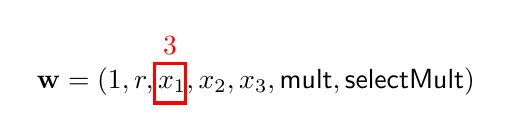
\begin{tikzpicture}
                % Node to contain the pmatrix
                \node (A) at (0,0) {$\mathbf{w} = (1, r, x_1, x_2, x_3, \mathsf{mult}, \mathsf{selectMult})$};
            
                \pause
                % Draw the red rectangle around the third column
                \draw[red, very thick] 
                    ([xshift=-108pt,yshift=-2pt]A.north east) -- ++(0,-0.5) -- 
                    ++(-0.4,0) -- ++(0,0.5) -- cycle;

                \node[xshift=-31pt,yshift=13pt,text=red] (B) at (0,0) {3};
            \end{tikzpicture}
        \end{center}
        \vspace{-8pt}
        Let's take a closer look at the matrix columns:
        \vspace{-8pt}
        \begin{center}
            \begin{tikzpicture}
                % Node to contain the pmatrix
                \node (A) at (0,0) {$
                    \begin{bmatrix}
                        0 & 0 & 1 & 0 & 0 & 0 & 0 \\
                        0 & 0 & 0 & 1 & 0 & 0 & 0 \\
                        0 & 0 & 1 & 0 & 0 & 0 & 0 \\
                        1 & 0 & -1 & 0 & 0 & 0 & 0 \\
                    \end{bmatrix}
                $};
            
                % Draw the red rectangle around the third column
                \draw[red, very thick] 
                    ([xshift=-71pt,yshift=-2pt]A.north east) -- ++(0,-1.93) -- 
                    ++(-0.7,0) -- ++(0,1.93) -- cycle;

                \node[xshift=-16pt,yshift=35pt,text=red] (B) at (0,0) {3};
            \end{tikzpicture}
        \end{center}
        \vspace{-10pt}
        Consider 4th constraint: $(1 - x_1) \times (x_2 + x_3) = r - \mathsf{selectMult}$
        \vspace{-8pt}
        \begin{center}
            \begin{tikzpicture}
                % Node to contain the pmatrix
                \node (A) at (0,0) {$
                    \begin{bmatrix}
                        0 & 0 & 1 & 0 & 0 & 0 & 0 \\
                        0 & 0 & 0 & 1 & 0 & 0 & 0 \\
                        0 & 0 & 1 & 0 & 0 & 0 & 0 \\
                        1 & 0 & -1 & 0 & 0 & 0 & 0 \\
                    \end{bmatrix}
                $};
            
                % Draw the red rectangle around the third column
                \draw[red, very thick] 
                    ([xshift=-71pt,yshift=-2pt]A.north east) -- ++(0,-1.93) -- 
                    ++(-0.7,0) -- ++(0,1.93) -- cycle;

                \node[xshift=-16pt,yshift=35pt,text=red] (B) at (0,0) {3};

                \draw[blue!70!black, very thick] 
                    ([xshift=-7.75pt,yshift=-45pt]A.north east) -- ++(-4,0) -- 
                    ++(0,-0.42) -- ++(4,0) -- cycle;
    
                \node[xshift=-63pt,yshift=-20pt,text=blue!70!black] (B) at (0,0) {4};

                \draw[black, very thick] 
                    ([xshift=-71pt,yshift=-45pt]A.north east) -- ++(-0.7,0) -- 
                    ++(0,-0.42) -- ++(0.7,0) -- cycle;
            \end{tikzpicture}
        \end{center}
        \pause
        \vspace{-10pt}
        So, every column is a mapping of constraint number to a coefficient for the witness element.
    \end{frame}

    \begin{frame}
        As we know, such a mapping can be builds using Lagrange interpolation polynomial with the
        following formula:
        \vspace{-10pt}
        \begin{equation*}
            L(x) = \sum_{i=0}^{n} y_i \ell_i(x), \quad \ell_i(x) = \prod_{j=0, j \neq i}^{n} \frac{x-x_j}{x_i-x_j}.
            \vspace{-10pt}
        \end{equation*}  

        \pause
        There are $n$ columns and $m$ constraints. So, it results in $n$ polynomials such that:
        \vspace{-10pt}
        \begin{equation*}
            A_j(i) = a_{i,j}, \; i \in \{1,2,\dots,m\}, \; j \in \{1,2,\dots,n\}
            \vspace{-10pt}
        \end{equation*}

        \pause
        The same is true for matrices $B$ and $C$, with $3n$ polynomials in total, $n$ for each of the
        coefficients matrices:
        \vspace{-8pt}
        \begin{align*}
            A_1(x), A_2(x), \dots, A_n(x), 
            B_1(x), B_2(x), \dots, B_n(x),
            C_1(x), C_2(x), \dots, C_n(x)
            \vspace{-10pt}
        \end{align*}

        \vspace{-10pt}
        \pause
        \begin{block}{Note}
            We could have assigned any \textit{unique} index from $\mathbb{F}$ to each constraint
            (say, $t_i$ for each $i \in \{1,\dots,m\}$) and interpolate through these points:
            \vspace{-8pt}
            \begin{equation*}
                A_j(t_i) = a_{i,j}, \; i \in \{1,2,\dots,m\}, \; j \in \{1,2,\dots,n\}
            \end{equation*}
        \end{block}
    \end{frame}

    \begin{frame}
        \begin{example}
            Considering the witness vector $\mathbf{w}$ and matrix $A$ from the previous example, for the variable
            $x_1$, the next set of points can be derived:
            \vspace{-10pt}
            \begin{equation*}
                \{(1,1), (2,0), (3,1), (4,-1)\}
            \end{equation*}
            The Lagrange interpolation polynomial for this set of points:
            \begin{align*}
                \ell_1(x) &= -\frac{(x - 2)(x - 3)(x - 4)}{6}, \quad &\ell_2(x) &= \frac{(x - 1)(x - 3)(x - 4)}{2}, \\
                \ell_3(x) &= -\frac{(x - 1)(x - 2)(x - 4)}{2}, \quad &\ell_4(x) &= \frac{(x - 1)(x - 2)(x - 3)}{6}.
            \end{align*}

            Thus, the polynomial is given by:
            \begin{align*}
                A_{x_1}(x) &= 1 \cdot \ell_1(x) + 0 \cdot \ell_2(x) + 1 \cdot \ell_3(x) + (-1) \cdot \ell_4(x) \\
                &= -\frac{5}{6}x^3 + 6x^2 - \frac{79}{6}x + 9
            \end{align*}
        \end{example}
    \end{frame}

    \begin{frame}
        \begin{center}
            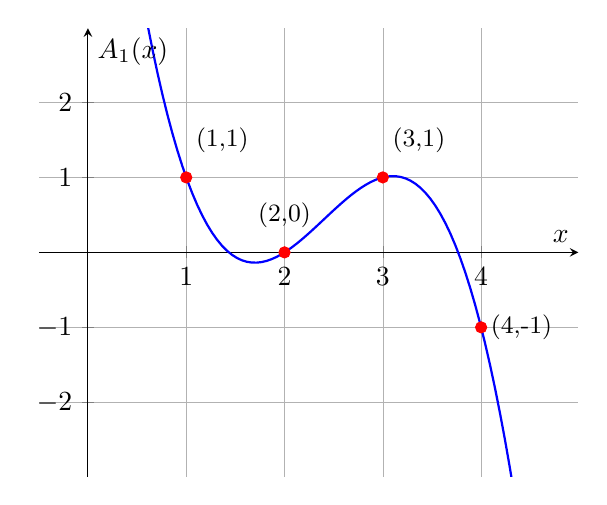
\begin{tikzpicture}
                \begin{axis}[
                    axis lines = middle,
                    xlabel = {$x$},
                    ylabel = {$A_1(x)$},
                    ymin = -2.99, ymax = 2.99,
                    xmin = -0.5, xmax = 4.99,
                    domain = 0:5,
                    samples = 100,
                    ytick = {-3,...,3},
                    xtick = {0,1,...,5},
                    grid = both, 
                    grid style = {line width=.1pt, draw=gray!20},
                    major grid style = {line width=.2pt, draw=gray!60}
                ]
                \addplot[
                    color=blue,
                    thick
                ]
                {-5/6*x^3 + 6*x^2 - 79/6*x + 9};
                \addplot[
                    only marks,
                    mark=*,
                    color=red
                ]
                coordinates {(1,1) (2,0) (3,1) (4,-1)};
        
                \node at (axis cs:1,1.5) [anchor=west] {\small (1,1)};
                \node at (axis cs:2,0.2) [anchor=south] {\small (2,0)};
                \node at (axis cs:3,1.5) [anchor=west] {\small (3,1)};
                \node at (axis cs:4,-1) [anchor=west] {\small (4,-1)};
                
                \end{axis}
            \end{tikzpicture}
    
            \scriptsize\textbf{Illustration:} The Lagrange inteprolation polynomial for points $\{(1,1), (2,0), (3,1), (4,-1)\}$ visualized over $\mathbb{R}$.
        \end{center}
    \end{frame}

    \begin{frame}
        \begin{alertblock}{Question}
            But what does it change? We ``exchanged`` $3n$ columns for $3n$ polynomials.
        \end{alertblock}

        \pause
        \vspace{-5pt}
        Consider two polynomials $p(x)$ and $q(x)$:
        \begin{equation*}
            \quad p(x) = -\frac{1}{2}x^2 + \frac{3}{2}x, \qquad
            q(x) = \frac{1}{3}x^3 - 2x^2 + \frac{8}{3}x + 1.
            \vspace{-5pt}
        \end{equation*}
        With corresponding sets of points:
        \vspace{-5pt}
        \begin{equation*}
            \{(0, 0), (1, 1), (2, 1), (3, 0)\}, \quad \{(0, 1), (1, 2), (2, 1), (3, 0)\}
            \vspace{-10pt}
        \end{equation*}
        
        \pause
        The sum of these polynomials can be calculated as:
        \vspace{-5pt}
        \begin{equation*}
            r(x) = \frac{1}{3}x^3 - 2\frac{1}{2}x^2 + 4\frac{1}{6}x + 1
            \vspace{-5pt}
        \end{equation*}
        The resulting polynomial $r(x)$ corresponds to the set of points:
        \vspace{-5pt}
        \begin{equation*}
            \{(0, 1), (1, 3), (2, 2), (3, 0)\}
        \end{equation*}
    \end{frame}

    \begin{frame}
        \begin{figure}[H]
            \centering
            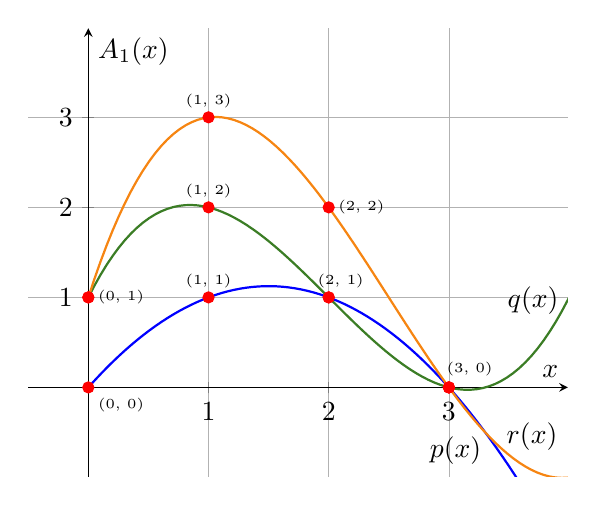
\begin{tikzpicture}
                \begin{axis}[
                    axis lines = middle,
                    xlabel = {$x$},
                    ylabel = {$A_1(x)$},
                    ymin = -0.99, ymax = 3.99,
                    xmin = -0.5, xmax = 3.99,
                    domain = 0:5,
                    samples = 100,
                    ytick = {-1,...,4},
                    xtick = {0,1,...,4},
                    grid = both,
                    grid style = {line width=.1pt, draw=gray!20},
                    major grid style = {line width=.2pt, draw=gray!60}
                ]

                % p(x)
                \addplot[
                    color=blue,
                    thick
                ]
                {3/2*x - 1/2*x^2};
                \addplot[
                    only marks,
                    mark=*,
                    color=red
                ]
                coordinates {(0, 0) (1, 1) (2, 1) (3, 0)};
                \node at (axis cs:3.35,-0.7) [anchor=east] {\text{$p(x)$}};

                \node at (axis cs:0,-0.2) [anchor=west] {\tiny (0, 0)};
                \node at (axis cs:1,1) [anchor=south] {\tiny (1, 1)};
                \node at (axis cs:2.1,1) [anchor=south] {\tiny (2, 1)};
                \node at (axis cs:2.9,0.2) [anchor=west] {\tiny (3, 0)};

                % q(x)
                \addplot[
                    color=OliveGreen,
                    thick
                ]
                {1/3*x^3 - 2*x^2 + 8/3*x + 1};
                \addplot[
                    only marks,
                    mark=*,
                    color=red
                ]
                coordinates {(0,1) (1,2) (2,1) (3, 0)};
                \node at (axis cs:3.7,0.7) [anchor=south] {\text{$q(x)$}};

                \node at (axis cs:0,1) [anchor=west] {\tiny (0, 1)};
                \node at (axis cs:1,2) [anchor=south] {\tiny (1, 2)};

                % r(x)
                \addplot[
                    color=BurntOrange,
                    thick
                ]
                {1/3*x^3 - 5/2*x^2 + 25/6*x + 1};
                \addplot[
                    only marks,
                    mark=*,
                    color=red
                ]
                coordinates {(0,1) (1,3) (2,2) (3, 0)};
                \node at (axis cs:3.4,-0.55) [anchor=west] {\text{$r(x)$}};

                \node at (axis cs:1,3) [anchor=south] {\tiny (1, 3)};
                \node at (axis cs:2,2) [anchor=west] {\tiny (2, 2)};

                \end{axis}
            \end{tikzpicture}
            \caption{Addition of two polynomials}
            \label{fig:example-polynomial-addition}
        \end{figure}
    \end{frame}

    \begin{frame}
        \vspace{-5pt}
        Now, using coefficients encoded with polynomials, we can build a constraint number 
        $X \in \{1, \dots\ m\}$ in the next way:
        \vspace{-5pt}
        \begin{align*}
            &(w_1A_1(X) + w_2A_2(X) + \dots + w_nA_n(X)) \times \\
            \times &(w_1B_1(X) + w_2B_2(X) + \dots + w_nB_n(X)) = \\ 
            = &(w_1C_1(X) + w_2C_2(X) + \dots + w_nC_n(X))
            \vspace{-5pt}
        \end{align*}
        \pause
        Or written more concisely:
        \vspace{-5pt}
        \begin{equation*}
            \left( \sum_{i = 1}^{n} w_iA_i(X) \right) \times \left( \sum_{i = 1}^{n} w_iB_i(X) \right) = \left( \sum_{i = 1}^{n} w_iC_i(X) \right)
        \end{equation*}        
    \end{frame}

    \begin{frame}
        Hold on, but why does it hold? Let us substitute any $X=j$ into this equation:
        \vspace{-5pt}
        \begin{equation*}
            \left( \sum_{i = 1}^{n} w_iA_i(j) \right) \times \left( \sum_{i = 1}^{n} w_iB_i(j) \right) = \left( \sum_{i = 1}^{n} w_iC_i(j) \right) \; \forall j \in \{1,\dots,m\}
            \vspace{-5pt}
        \end{equation*}
        \pause
        Recall that we interpolated polynomials to have $A_i(j) = a_{j,i}$. Therefore, the equation above can be reduced to:
        \vspace{-5pt}
        \begin{equation*}
            \left( \sum_{i = 1}^{n} w_ia_{j,i} \right) \times \left( \sum_{i = 1}^{n} w_ib_{j,i} \right) = \left( \sum_{i = 1}^{n} w_ic_{j,i} \right) \; \forall j \in \{1,\dots,m\}
            \vspace{-5pt}
        \end{equation*}
        \pause
        But hold on again! Notice that $\sum_{i = 1}^{n} w_ia_{j,i} = \langle \mathbf{w}, \mathbf{a}_j \rangle$ and therefore we have:
        \vspace{-5pt}
        \begin{equation*}
            \langle \mathbf{w}, \mathbf{a}_j \rangle \times \langle \mathbf{w}, \mathbf{b}_j \rangle = \langle \mathbf{w}, \mathbf{c}_j \rangle \; \forall j \in \{1,\dots,m\},
            \vspace{-5pt}
        \end{equation*}
        
        so we ended up with the initial $m$ constraint equations!       
    \end{frame}

    \begin{frame}
        Now let us define polynomials $A(X)$, $B(X)$, $C(X)$ for easier notation: 
        \vspace{-5pt}
        \begin{equation*}
            A(X) = \sum_{i = 1}^{n} w_iA_i(X), \quad B(X) = \sum_{i = 1}^{n} w_iB_i(X), \quad C(X) = \sum_{i = 1}^{n} w_iC_i(X)
            \vspace{-5pt}
        \end{equation*}
        \pause  
        Therefore:
        \vspace{-5pt}
        \begin{equation*}
            A(X) \times B(X) = C(X)
            \vspace{-5pt}
        \end{equation*}

        Now, we can define a polynomial $M(X)$, that has zeros at all elements from the set
        $\Omega = \{1,\dots,m\}$
        \vspace{-5pt}
        \begin{equation*}
            M(X) = A(X) \times B(X) - C(X)
            \vspace{-5pt}
        \end{equation*}
        \pause
        It means, that $M(X)$ can be devide by \textbf{vanishing polynomial} $Z_{\Omega}(X)$ without a remainder!
        \vspace{-8pt}
        \begin{equation*}
            Z_{\Omega}(X) = \prod_{i=1}^m (X - i), \qquad H(X) = \frac{M(X)}{Z_{\Omega}(X)}
            \vspace{-5pt}
        \end{equation*}
    \end{frame}

    \begin{frame}
        \begin{definition}[Quadratic Arithmetic Program]
            Suppose that $m$ R1CS constraints with a witness of size $n$ are written in a form
            \begin{equation*}
                A\mathbf{w} \odot B\mathbf{w} = C\mathbf{w}, \; A,B,C \in \mathbb{F}^{m \times n}
            \end{equation*}
        
            Then, the \textbf{Quadratic Arithmetic Program} consists of $3n$ polynomials $A_1,\dots,A_n$, $B_1,\dots,B_n$, $C_1,\dots,C_n$ such that:
            \begin{equation*}
                A_j(i) = a_{i,j}, \; B_j(i) = b_{i,j}, \; C_j(i) = c_{i,j}, \; \forall i \in \{1,\dots,m\} \; \forall j \in \{1,\dots,n\}
            \end{equation*}
        
            Then, $\mathbf{w} \in \mathbb{F}^n$ is a valid assignment for the given QAP and \textbf{target polynomial} $Z(X) = \prod_{i=1}^m (X-i)$ if and only if there exists such a polynomial $H(X)$ such that
            \begin{equation*}
                \left( \sum_{i = 1}^{n} w_iA_i(X) \right)\left( \sum_{i = 1}^{n} w_iB_i(X) \right) - \left( \sum_{i = 1}^{n} w_iC_i(X) \right) = Z(X)H(X)
            \end{equation*}
        \end{definition}
    \end{frame}

    \section{Probabilistically Checkable Proofs}

    \begin{frame}
        \begin{figure}[H]
            \centering
            \begin{tikzpicture}
                \node[inner sep=0pt, align=center] at (-4.0, 0.0) (prover) {
\includegraphics[width=1.25cm]{images/common/prover.png}\\Prover $\mathcal{P}$};
                \node[inner sep=0pt, align=center] at (4.0, 0.0) (verifier) {
\includegraphics[width=1.25cm]{images/common/verifier.png}\\Verifier $\mathcal{V}$};
        
                \draw[fill=gray!20!white, ultra thick] (-2.0, 4) rectangle (2.0, 3.25);
        
                \node at (0, 2.85) (pcp) {\textbf{PCP Oracle}};
                \draw[-{Stealth[length=3mm]},line width=0.4mm] (prover)--(pcp) node[midway, left=3mm]{Generate an oracle ($\pi$)};
                \draw[-{Stealth[length=3mm]},line width=0.4mm] (verifier)--(pcp) node[midway, right=3mm]{Point queries $q_1,\dots,q_m$};

                \pause
                % Query boxes
                \draw[fill=blue!60!white, ultra thick] (-1.0, 4) rectangle (-0.8, 3.25);
                \node at (-0.9, 4.35) (pcp) {$q_1$};
                \draw[fill=blue!60!white, ultra thick] (0.0, 4) rectangle (0.2, 3.25);
                \node at (0.1, 4.35) (pcp) {$q_2$};
                \draw[fill=blue!60!white, ultra thick] (0.5, 4) rectangle (0.7, 3.25);
                \node at (0.6, 4.35) (pcp) {$q_3$};
            \end{tikzpicture}
            \caption{Illustration of a Probabilistically Checkable Proof (PCP) system. The prover $\mathcal{P}$ generates a PCP oracle $\pi$ that is queried by the verifier $\mathcal{V}$ at specific points $q_1,\dots,q_m$.}
        \end{figure}
    \end{frame}

    \begin{frame}
        Three main extensions of PCPs that are frequently used in SNARKs are:
        \begin{itemize}
            \item \textbf{IPCP} (\textbf{Interactive PCP}): The prover commits to the PCP oracle and then, based on the interaction between the prover and verifier, the verifier queries the oracle and decides whether to accept the proof.
            \item \textbf{IOP} (\textbf{Interactive Oracle Proof}): The prover and verifier interact and on each round, the prover commits to a new oracle. The verifier queries the oracle and decides whether to accept the proof.
            \item \textbf{LPCP} (\textbf{Linear PCP}): The prover commits to a linear function and the verifier queries the function at specific points.
        \end{itemize}
    \end{frame}

    \begin{frame}
        \begin{figure}[H]
            \centering
            \begin{tikzpicture}
                \node[inner sep=0pt, align=center] at (-4.0, 0.5) (prover) {
\includegraphics[width=1cm]{images/common/prover.png}\\Prover $\mathcal{P}$};
                \node[inner sep=0pt, align=center] at (4.0, 0.5) (verifier) {
\includegraphics[width=1cm]{images/common/verifier.png}\\Verifier $\mathcal{V}$};
        
                % Oracle 1
                \node at (-2.0, 5.625) (oracle_1_left) {};
                \node at (2.0, 5.625) (oracle_1_right) {};
                \draw[fill=gray!20!white, ultra thick] (-2.0, 6) rectangle (2.0, 5.25);
                \draw[fill=blue!60!white, ultra thick] (-1.0, 6) rectangle (-0.8, 5.25);
                \node at (-0.9, 6.35) (pcp) {$q_1$};
                \draw[fill=blue!60!white, ultra thick] (0.0, 6) rectangle (0.2, 5.25);
                \node at (0.1, 6.35) (pcp) {$q_2$};
                \draw[fill=blue!60!white, ultra thick] (0.5, 6) rectangle (0.7, 5.25);
                \node at (0.6, 6.35) (pcp) {$q_3$};
                \node at (0, 4.85) (pcp) {\textbf{PCP Oracle \#1}};
        
                % Oracle 2
                \node at (-2.0, 3.625) (oracle_2_left) {};
                \node at (2.0, 3.625) (oracle_2_right) {};
                \draw[fill=gray!20!white, ultra thick] (-2.0, 4) rectangle (2.0, 3.25);
                \draw[fill=blue!60!white, ultra thick] (-0.4, 4) rectangle (-0.2, 3.25);
                \node at (-0.3, 4.35) (pcp) {$q_1'$};
                \draw[fill=blue!60!white, ultra thick] (0.2, 4) rectangle (0.4, 3.25);
                \node at (0.3, 4.35) (pcp) {$q_2'$};
                \draw[fill=blue!60!white, ultra thick] (1.5, 4) rectangle (1.7, 3.25);
                \node at (1.6, 4.35) (pcp) {$q_3'$};
                \node at (0, 2.85) (pcp) {\textbf{PCP Oracle \#2}};
        
                % Oracle 3
                \node at (-2.0, 1.625) (oracle_3_left) {};
                \node at (2.0, 1.625) (oracle_3_right) {};
                \draw[fill=gray!20!white, ultra thick] (-2.0, 2) rectangle (2.0, 1.25);
                \draw[fill=blue!60!white, ultra thick] (-1.5, 2) rectangle (-1.3, 1.25);
                \node at (-1.4, 2.35) (pcp) {$q_1''$};
                \draw[fill=blue!60!white, ultra thick] (0.3, 2) rectangle (0.5, 1.25);
                \node at (0.4, 2.35) (pcp) {$q_2''$};
                \draw[fill=blue!60!white, ultra thick] (1.0, 2) rectangle (1.2, 1.25);
                \node at (1.1, 2.35) (pcp) {$q_3''$};
                \node at (0, 0.85) (pcp) {\textbf{PCP Oracle \#3}};
        
                \draw[-{Stealth[length=3mm]},line width=0.4mm] (prover)--(oracle_1_left) node[midway, left=3mm]{\shortstack{Commit to\\oracles}};
                \draw[-{Stealth[length=3mm]},line width=0.4mm] (verifier)--(oracle_1_right) node[midway, right=3mm]{Point queries};
                \draw[-{Stealth[length=3mm]},line width=0.4mm] (prover)--(oracle_2_left) node[midway, left=3mm]{};
                \draw[-{Stealth[length=3mm]},line width=0.4mm] (verifier)--(oracle_2_right) node[midway, right=3mm]{};
                \draw[-{Stealth[length=3mm]},line width=0.4mm] (prover)--(oracle_3_left) node[midway, left=3mm]{};        
                \draw[-{Stealth[length=3mm]},line width=0.4mm] (verifier)--(oracle_3_right) node[midway, right=3mm]{};
        
                % Two arrows to left and to right between the prover and verifier with the "Interaction" label
                \draw[{Stealth[length=3mm]}-{Stealth[length=3mm]},line width=0.4mm,dashed] (prover) to node[midway, below]{Interaction} (verifier);
            \end{tikzpicture}
            \caption{Illustration of an Interactive Oracle Proof (IOP). On each round $i$ ($1 \leq i \leq r$), $\mathcal{V}$ sends a message $m_i$, and $\mathcal{P}$ commits to a new oracle $\pi_i$, which $\mathcal{V}$ can query at $\mathbf{q}_i=(q_{i,1},\dots,q_{i,m})$.}
            \label{fig:pcp}
        \end{figure}
    \end{frame}

    \section{QAP as a Linear PCP}

    \begin{frame}
        \begin{definition}[Linear PCP]
            A \textbf{Linear PCP} is a PCP where the prover commits to a linear function $\boldsymbol{\pi} = (\pi_1,\dots,\pi_k)$ and the verifier queries the function at specific points $\boldsymbol{q}_1,\dots,\boldsymbol{q}_r$. Then, the prover responds with the values of the function at these points:
            \begin{equation*}
                \langle \boldsymbol{\pi}_1, \mathbf{q}_1 \rangle, \langle \boldsymbol{\pi}_2, \mathbf{q}_2 \rangle, \dots, \langle \boldsymbol{\pi}_r, \mathbf{q}_r \rangle.
            \end{equation*}
        \end{definition}
    \end{frame}

    \begin{frame}
        \begin{example}[QAP as a Linear PCP]
            Recall that key QAP equation is:
            \begin{equation*}
                L(x) \times R(x) - O(x) = Z(x)H(x).
            \end{equation*}
            
            Now, consider the following \textbf{linear PCP for QAP}:
            \begin{enumerate}
                \item $\mathcal{P}$ commits to an extended witness $\mathbf{w}$ and coefficients $\mathbf{h} = (h_1,\dots,h_n)$ of $H(x)$.
                \item $\mathcal{V}$ samples $\gamma \xleftarrow{R} \mathbb{F}$ and sends query $\boldsymbol{\gamma} = (\gamma,\gamma^2,\dots,\gamma^n)$ to $\mathcal{P}$.
                \item $\mathcal{P}$ reveals the following values:
                \begin{align*}
                    \pi_1 &\gets \langle \mathbf{w}, \boldsymbol{L}(\gamma) \rangle, \quad &\pi_2 &\gets \langle \mathbf{w}, \boldsymbol{R}(\gamma) \rangle, \\ 
                    \pi_3 &\gets \langle \mathbf{w}, \boldsymbol{O}(\gamma) \rangle, \quad &\pi_4 &\gets Z(\gamma) \cdot \langle \mathbf{h}, \boldsymbol{\gamma} \rangle.
                \end{align*}
                \item $\mathcal{V}$ checks whether $\pi_1\pi_2 - \pi_3 = \pi_4$.
            \end{enumerate}
        \end{example}
    \end{frame}

    \begin{frame}{}
        \centering \Large
        \emph{Thanks for your attention!}
    \end{frame}
\end{document}